\begin{frame}{Efficiencies and false positive rates}
\begin{columns}
\column{.5\textwidth}
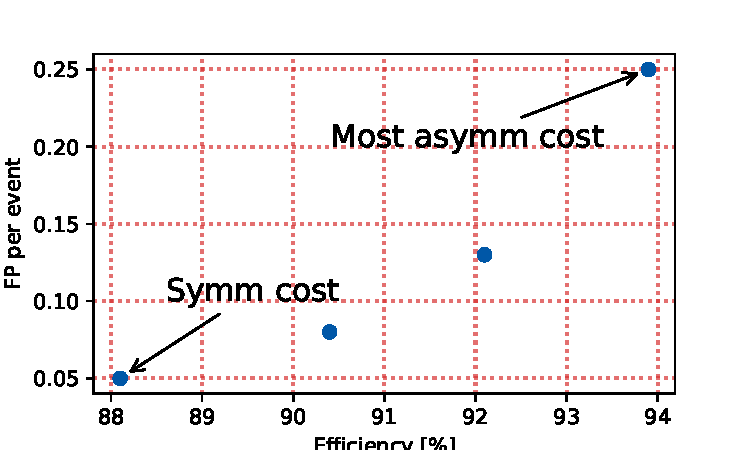
\includegraphics[width=\textwidth]{images/EffVsFP.pdf}
\column{.5\textwidth}
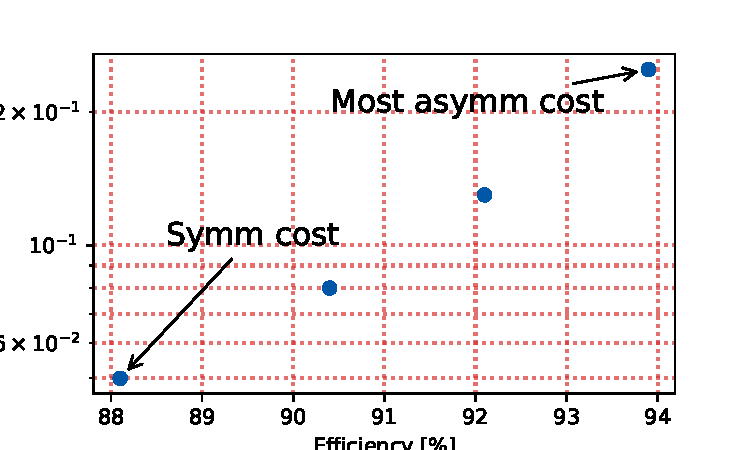
\includegraphics[width=\textwidth]{images/EffVsFP_semilog.pdf}
\end{columns}

  \begin{columns}
      \column{.5\textwidth}
  \begin{block}{Search for PVs}
    \begin{itemize}
    	\item Search $ \pm 5 $ bins ($ \pm 500 \mu $m) around a true PV
    	\item At least 3 bins with predicted probability
    	   $ > 1\% $ and
    	   integrated probability $ > 20\%$.
    \end{itemize}
    \end{block}

    \column{.5\textwidth}
    \begin{block}{Tunable efficiency vs. FP}
    \begin{itemize}
        \item The asymmetry parameter controls efficiency vs. FP
    \end{itemize}
  \end{block}
\end{columns}
\end{frame}
